\begin{figure}[H]
	\centering
	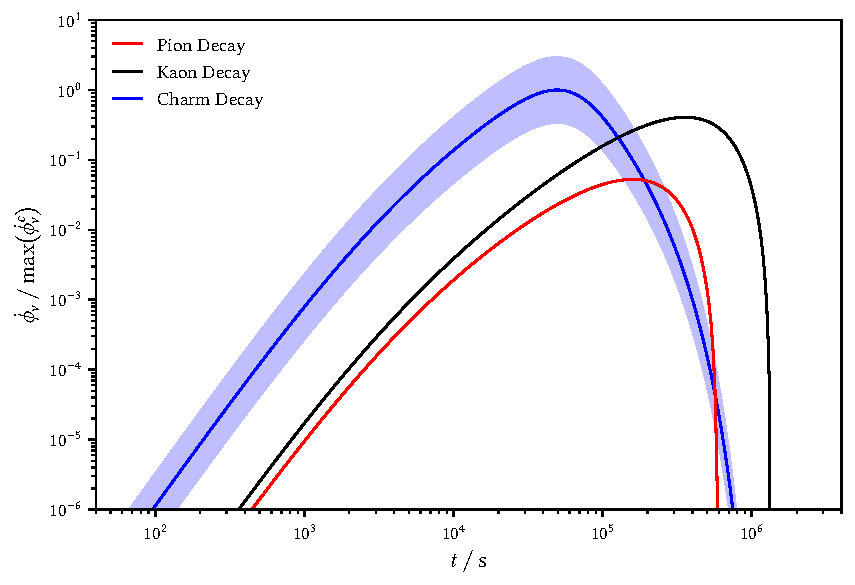
\includegraphics{../plots/build/magnetar_neutrino_spectrum_without.pdf}
	\caption[Magnetar $\nu \kern+0.5pt$ flux compared to $c$ decay without optical depth.]
			{Effective neutrino light curves normalized to the maximum charm decay flux at
			 $E_\nu = \kern-0.5pt \qty{e9}{\giga\electronvolt}$ from a newborn magnetar, excluding the optical depth
			 defined by \eqref{eqn:optical} as a modification. Properties of hadronic components in agreement with
			 Figure \ref{fig:magnetar-flux-with} are observed. The different shapes that are also seen in Figure
			 \ref{fig:magnetar-charm-comparison-without} agree with cooling and the omission of an optical depth 
			 as described in Section \ref{sub:cooling} and lead to pion and charm peaks with larger magnitudes.
			 The same shaded uncertainty band as in Figure \ref{fig:magnetar-flux-with} is adopted for charm decays.}
	\label{fig:magnetar-flux-without}
\end{figure}
